% =============================================================================
% CalRank (Conference Version) — 6-page IEEE format
% Compile: pdflatex calrank_conference.tex
%
% Uses IEEEtran class. If unavailable on your system, Overleaf provides it
% under the "IEEE Official Templates" gallery.
% =============================================================================
\documentclass[conference]{IEEEtran}

\usepackage[utf8]{inputenc}
\usepackage[T1]{fontenc}
\usepackage{amsmath,amssymb}
\usepackage{graphicx}
\usepackage{booktabs}
\usepackage{multirow}
\usepackage{array}
\usepackage{siunitx}
\usepackage[table]{xcolor}
\usepackage[hidelinks]{hyperref}
\usepackage{cite}
\usepackage{microtype}
\usepackage{enumitem}

\graphicspath{{../data/figures/}}

\sisetup{detect-weight=true,detect-family=true}
\newcommand{\ece}{\mathrm{ECE}}
\newcommand{\sigmoid}{\sigma}

% Table colours
\definecolor{headblue}{HTML}{2C3E6B}
\definecolor{rowlight}{HTML}{EAF0FA}
\definecolor{rowwhite}{HTML}{FFFFFF}
\definecolor{cleangreen}{HTML}{E6F5E8}
\definecolor{singleclasspink}{HTML}{FDE8E8}
\newcommand{\thead}[1]{\textcolor{white}{\textbf{#1}}}

\title{How Calibrated Are Cross-Encoder Re-Rankers?\\
An Empirical Study and a Cautionary Tale}

\author{
  \IEEEauthorblockN{Sayanjib [Surname]}
  \IEEEauthorblockA{[Affiliation]\\
  [City, Country]\\
  \texttt{[email]}}
}

\begin{document}
\maketitle

% =============================================================================
\begin{abstract}
Cross-encoder re-rankers are increasingly used as probability estimators in
retrieval-augmented generation pipelines, abstention layers, and multi-stage
cascades, yet nobody has systematically checked whether their sigmoid scores
are calibrated. We measure Expected Calibration Error (ECE), Maximum
Calibration Error, and Brier score for five cross-encoders (4M--278M
parameters) across nine BEIR domains. Every model is overconfident, with
optimal temperatures ranging from 3 to above 20. We also identify a
methodological hazard: five of nine BEIR datasets carry only positive
judgments, which silently corrupts calibration evaluation and makes
temperature scaling appear unreliable when it is not. Restricting to datasets
with genuine negatives, we find that isotonic regression, Platt scaling, and
temperature scaling all reduce calibration error substantially, none of them
disturb the ranking, and a clear ordering emerges (isotonic $>$ Platt $>$
temperature). We release scored pairs, fitted calibrators, and code.
\end{abstract}

\begin{IEEEkeywords}
calibration, cross-encoder re-ranking, ECE, temperature scaling, isotonic
regression, BEIR, retrieval-augmented generation
\end{IEEEkeywords}

% =============================================================================
\section{Introduction}
\label{sec:intro}

A cross-encoder re-ranker reads a query alongside a candidate document and
produces a score. Sort by score and you have a ranking. That much is
well-understood. What is newer, and less examined, is the growing practice of
treating that score as a probability. A retrieval-augmented assistant might
forward only passages scoring above $p=0.7$ to its generator~\cite{lewis2020rag}.
An abstention system might refuse to answer when nothing in the pool looks
confident enough. A cascade might route low-confidence queries to a bigger
model~\cite{gao2024rag}. In each case, $\sigmoid(\text{logit})$ is consumed
as $P(\text{relevant}\mid q,d)$.

Whether that trust is warranted is an open question. These models learn from
MS~MARCO~\cite{nguyen2016msmarco} with ranking objectives. Separation is what
matters during training: relevant above non-relevant. Probabilistic accuracy
is a different property entirely~\cite{degroot1983}, and a model can excel at
one while failing at the other. The calibration literature has covered image
classifiers~\cite{guo2017} and large language models~\cite{kadavath2022}, but
cross-encoder re-rankers, despite serving as de facto probability estimators
in production, have mostly escaped scrutiny.

We set out to fill that gap and, in the process, stumbled onto a second
problem: a structural issue with how calibration is evaluated on standard IR
benchmarks. Our contributions are:

\begin{itemize}[leftmargin=*,itemsep=1pt]
  \item \textbf{C1.} The first systematic calibration study of small
  cross-encoder re-rankers: five models across nine BEIR domains, with ECE,
  MCE, and Brier score supported by bootstrap confidence intervals.

  \item \textbf{C2.} Identification of a methodological hazard: five of nine
  datasets carry only positive judgments (prevalence = 1.0), which makes
  calibration evaluation degenerate and produces misleading method comparisons.

  \item \textbf{C3.} On datasets with genuine negatives, all three post-hoc
  methods work, with a clear ranking: isotonic $>$ Platt $>$ temperature.
  Ranking quality is preserved to within $10^{-4}$ in nDCG@10.

  \item \textbf{C4.} Release of scored pairs, fitted calibrators, and a
  deployment recipe.
\end{itemize}

% =============================================================================
\section{Related Work}
\label{sec:related}

The two-stage pipeline, BM25 followed by a cross-encoder, has become
standard~\cite{nogueira2019}. Nogueira and Cho fine-tuned BERT for passage
re-ranking, and the idea has since branched into distilled variants like
MiniLM~\cite{wang2020minilm} and TinyBERT~\cite{jiao2020tinybert},
architecturally distinct approaches like ELECTRA~\cite{clark2020electra}, and
multilingual models like BGE~\cite{xiao2023bge}. All share a single logit
output mapped through a sigmoid.

Calibration, the property that a predicted probability means what it
says~\cite{degroot1983}, is typically assessed via ECE~\cite{naeini2015} and
reliability diagrams~\cite{niculescu2005}. Temperature scaling~\cite{guo2017}
divides the logit by a learned scalar $T$; Platt scaling~\cite{platt1999}
fits a two-parameter logistic regression on the logit; isotonic
regression~\cite{zadrozny2002} learns a non-parametric monotone map. All
three preserve document ordering. Guo et al.\ showed that modern deep
networks are often more overconfident than shallower ones, and recent work
has extended calibration analysis to LLMs~\cite{kadavath2022,tian2023} and
NLI~\cite{desai2020}. In IR specifically, Craswell et al.~\cite{craswell2020}
and Lin et al.~\cite{lin2021pyserini} evaluated neural re-rankers on BEIR,
but their focus was ranking effectiveness, not whether the probability
estimates themselves are trustworthy. To our knowledge, no systematic
cross-domain calibration study of cross-encoder re-rankers exists.

% =============================================================================
\section{Methodology}
\label{sec:method}

\subsection{Models and Datasets}

We study five publicly available cross-encoders (Table~\ref{tab:models}),
spanning 4M to 278M parameters and covering distilled BERT variants,
ELECTRA, and XLM-RoBERTa. We intentionally confined ourselves to small
models because those are what engineers actually deploy in latency-sensitive
settings.

\begin{table}[t]
\centering
\caption{Cross-encoder re-rankers studied.}
\label{tab:models}
\scriptsize
\begin{tabular}{llrl}
\toprule
\rowcolor{headblue}
\thead{Key} & \thead{HuggingFace ID} & \thead{Params} & \thead{Arch.} \\
\midrule
\rowcolor{rowlight}
TinyBERT-L2  & ce/ms-marco-TinyBERT-L-2-v2 & 4M   & TinyBERT \\
\rowcolor{rowwhite}
MiniLM-L6    & ce/ms-marco-MiniLM-L-6-v2   & 22M  & MiniLM \\
\rowcolor{rowlight}
MiniLM-L12   & ce/ms-marco-MiniLM-L-12-v2  & 33M  & MiniLM \\
\rowcolor{rowwhite}
ELECTRA      & ce/ms-marco-electra-base     & 110M & ELECTRA \\
\rowcolor{rowlight}
BGE          & BAAI/bge-reranker-base       & 278M & XLM-R \\
\bottomrule
\end{tabular}
\vspace{-0.3cm}
\end{table}

We evaluate on nine BEIR-family datasets~\cite{thakur2021beir}
(Table~\ref{tab:datasets}), ordered by positive prevalence, the fraction of
judged pairs carrying a positive label. This ordering turns out to be the
most consequential dimension in the study. Four datasets contain genuine
negatives (prevalence $<1.0$); the remaining five have only positive
judgments, a fact that silently corrupts calibration evaluation
(Section~\ref{sec:hazard}).

\begin{table}[t]
\centering
\caption{Datasets ordered by prevalence.
\textcolor{green!50!black}{Green}: genuine negatives.
\textcolor{red!50!black}{Pink}: positive-only.}
\label{tab:datasets}
\scriptsize
\begin{tabular}{llrrr}
\toprule
\rowcolor{headblue}
\thead{Dataset} & \thead{Domain} & \thead{\#Q} & \thead{\#Judged} & \thead{Prev.} \\
\midrule
\rowcolor{cleangreen}
dbpedia-entity   & Entity          & 400   & 9{,}182 & 0.35 \\
\rowcolor{cleangreen}
trec-covid       & Biomedical      & 50    & 3{,}475 & 0.62 \\
\rowcolor{cleangreen}
webis-touche2020 & Argument        & 49    & 635     & 0.78 \\
\rowcolor{cleangreen}
scidocs          & Citation        & 1{,}000 & 1{,}774 & 0.95 \\
\rowcolor{singleclasspink}
arguana          & Counter-arg.    & 1{,}406 & 1{,}316 & 1.00 \\
\rowcolor{singleclasspink}
fiqa             & Financial QA    & 648   & 756     & 1.00 \\
\rowcolor{singleclasspink}
nfcorpus         & Health          & 323   & 1{,}941 & 1.00 \\
\rowcolor{singleclasspink}
quora            & Duplicates      & 1{,}000 & 1{,}278 & 1.00 \\
\rowcolor{singleclasspink}
scifact          & Claims          & 300   & 298     & 1.00 \\
\bottomrule
\end{tabular}
\vspace{-0.3cm}
\end{table}

\subsection{Pipeline and Metrics}

For each query we retrieve the top 100 documents via
BM25~\cite{robertson2009bm25} ($k_1{=}0.9$, $b{=}0.4$), then score every
candidate with all five cross-encoders. We compute ECE (15 equal-width
bins), MCE, and Brier score on judged pairs, with 95\% bootstrap CIs on ECE
(1{,}000 query-level resamples). Post-hoc calibrators (temperature, Platt,
isotonic) are fit on a 50/50 stratified split and evaluated on the held-out
half. No calibrator is ever evaluated on its training data.

% =============================================================================
\section{Results}
\label{sec:results}

\subsection{Universal Overconfidence}
\label{sec:overconf}

Figure~\ref{fig:heatmap} makes the scale of the problem clear. Warm colours
dominate: every model is overconfident on every domain where the measurement
is meaningful. Optimal temperatures range from about 3 (BGE on dbpedia) to
above 20 (fifteen of forty-five pairs hit the search ceiling). Think about
what $T{=}10$ means practically: you have to divide the logit by ten before
the sigmoid produces anything resembling a real probability. That is the
median situation, not an outlier.

One question we expected to answer cleanly was whether bigger models
calibrate better. They do not, at least in this size range. The Spearman
correlation between parameter count and mean raw ECE is $\rho = -0.10$
($p = 0.87$). MiniLM-L12 at 33M has the lowest mean ECE; BGE at 278M sits
near the middle.

\begin{figure}[t]
\centering
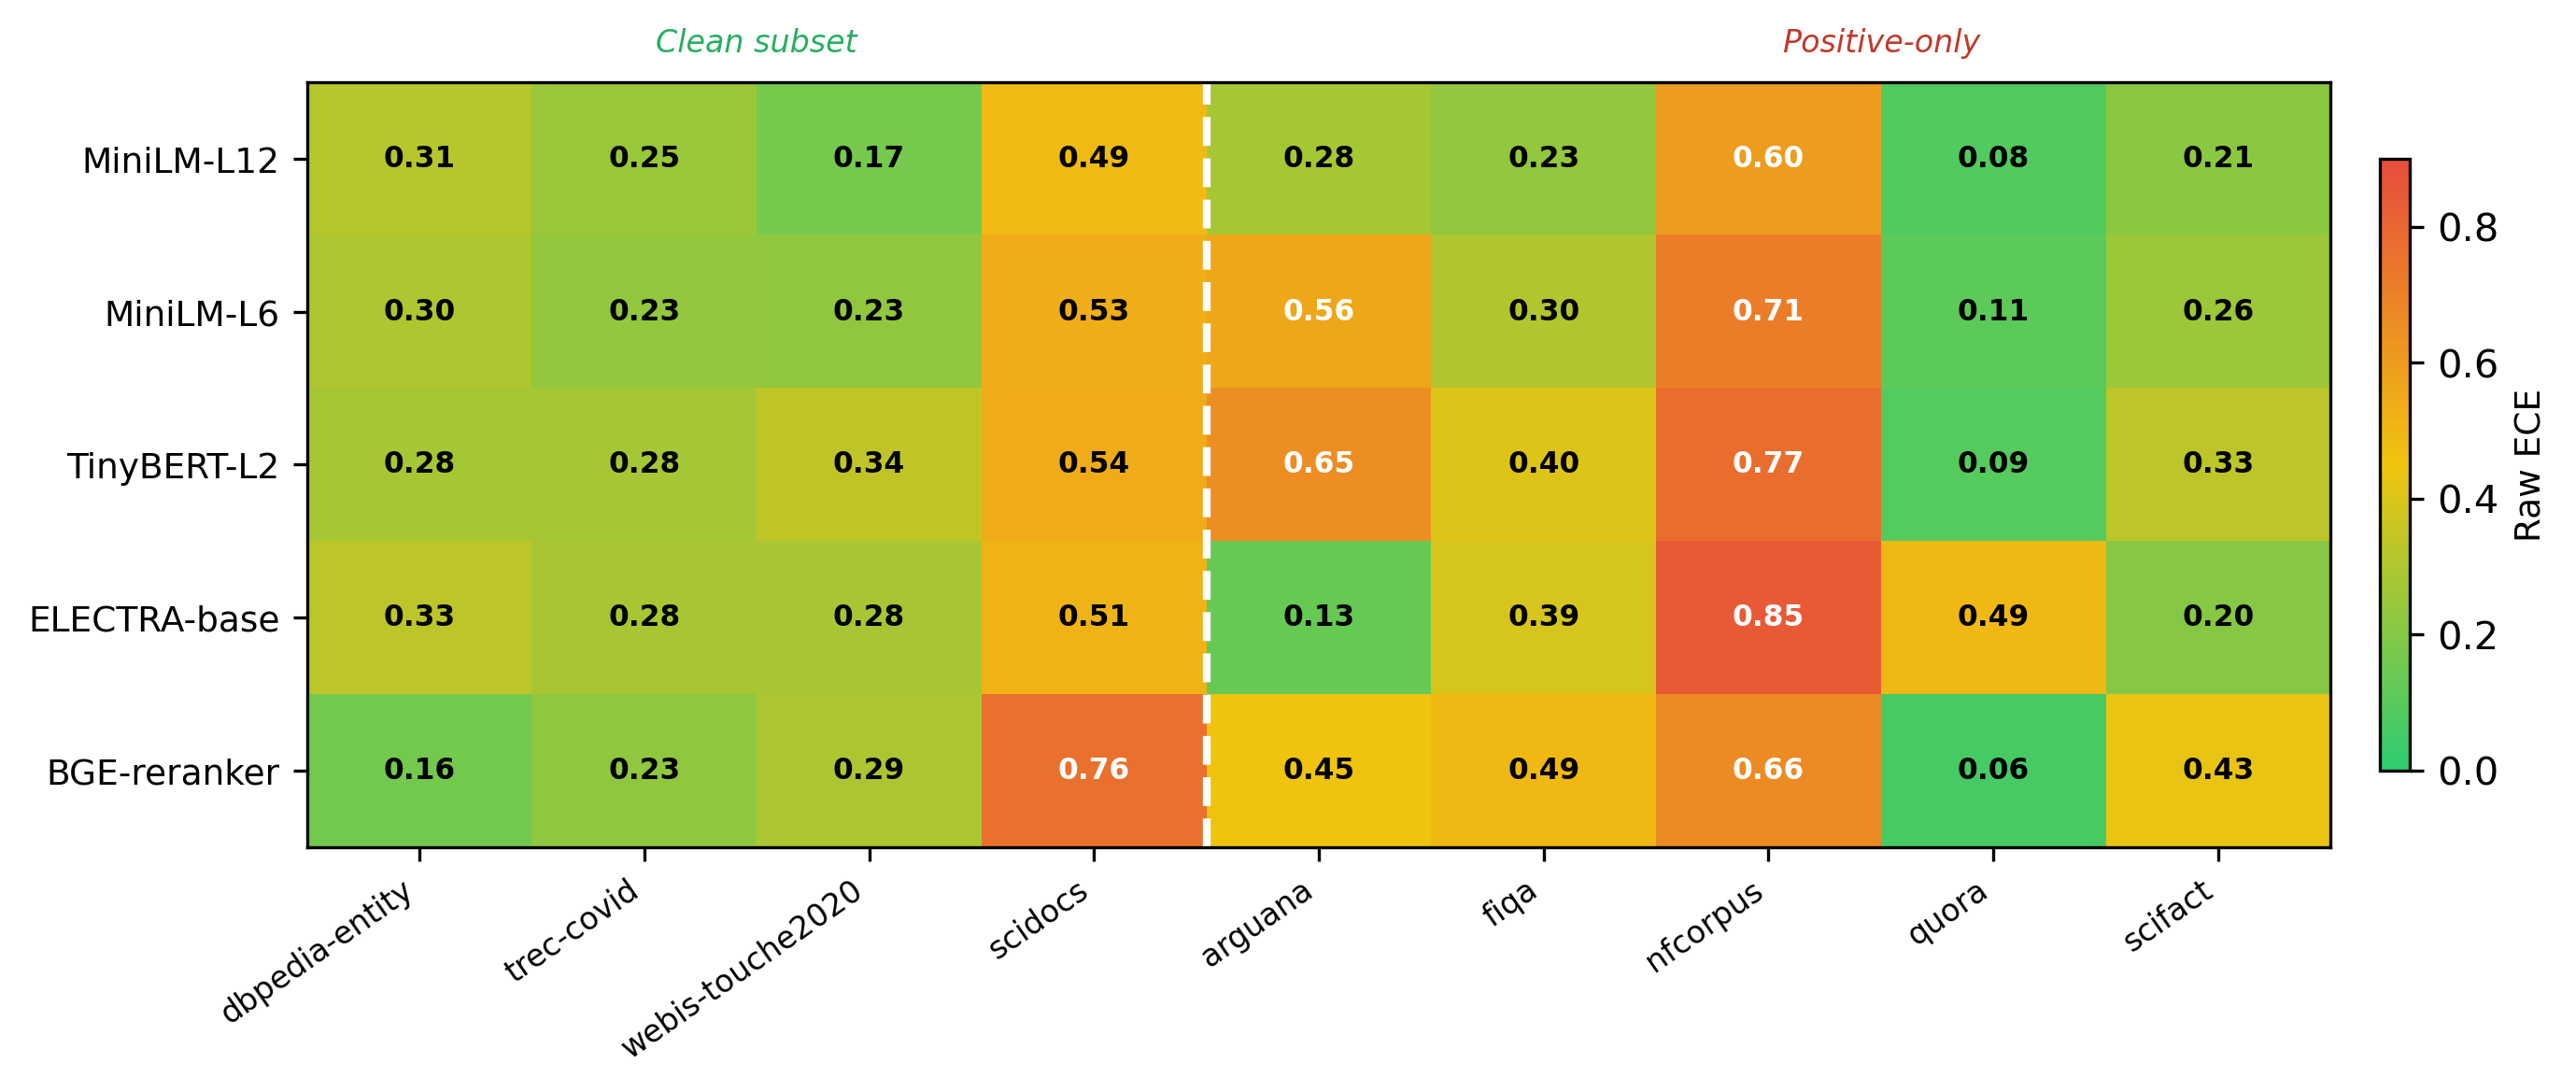
\includegraphics[width=\columnwidth]{paper_fig_ece_heatmap.png}
\caption{Raw ECE heatmap across all 45 model-dataset pairs. Green is low
error, red is high. The dashed line separates clean data (left) from
positive-only datasets (right). Overconfidence is the norm.}
\label{fig:heatmap}
\end{figure}

\subsection{The Hazard: Positive-Only Judgments Break Evaluation}
\label{sec:hazard}

This is the finding we think matters most. Five datasets have prevalence
exactly 1.0: every judged document is relevant. On such data, calibration
evaluation becomes degenerate. Isotonic regression maps everything to the
majority class and achieves ECE of 0.000, a number that looks spectacular
but is meaningless. Temperature scaling has no negative examples to learn
from, so the optimiser drifts or, worse, actively worsens calibration.
Figure~\ref{fig:backfire} shows this on scifact: temperature \emph{raises}
ECE while isotonic trivially zeros it. Neither number reflects genuine
calibration quality.

If you pool all 45 pairs naively, temperature appears unreliable
(improves only 27/45, $d{=}0.40$) while isotonic appears magical (improves
all 45). Both conclusions are wrong. The prevalence structure created them.

\begin{figure}[t]
\centering
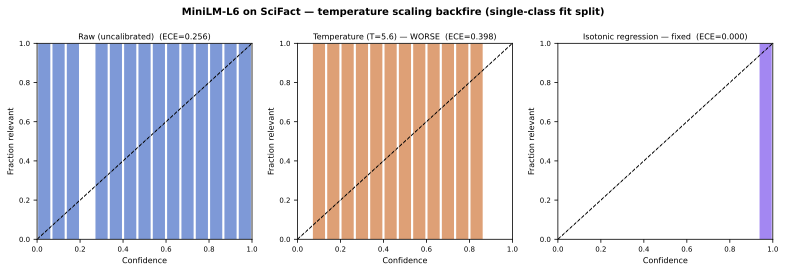
\includegraphics[width=\columnwidth]{paper_fig2_minilm_scifact_temp_backfire.png}
\caption{MiniLM-L6 on scifact (prevalence 1.0). Temperature scaling
\emph{worsens} ECE; isotonic regression trivially zeros it. Neither number
means anything without negative judgments.}
\label{fig:backfire}
\end{figure}

\subsection{On Clean Data, All Methods Work}
\label{sec:clean}

Restricting to the four datasets with genuine negatives gives twenty
model-dataset pairs. Here the picture changes substantially.
Table~\ref{tab:clean} reports aggregated results. Temperature scaling
improves all 20 pairs ($d{=}1.41$, $p{<}0.0001$), reducing mean ECE from
0.340 to 0.232. Platt scaling does considerably better (mean ECE 0.045,
$d{=}1.72$), and isotonic regression is best of all (mean ECE 0.025,
$d{=}2.02$). The jump from temperature to Platt is much larger than from
Platt to isotonic, which makes Platt an interesting practical sweet spot
when calibration sets are small.

Figure~\ref{fig:fixworks} shows the progression on a single clean example:
BGE on trec-covid. The bars move from well below the diagonal to nearly
touching it.

\begin{table}[t]
\centering
\caption{Calibration on the clean subset (4 datasets with genuine
negatives). Mean ECE across 20 model-dataset pairs, held-out split.}
\label{tab:clean}
\scriptsize
\begin{tabular}{lrrrr}
\toprule
\rowcolor{headblue}
\thead{Method} & \thead{mean ECE} & \thead{Improves} & \thead{$d$} & \thead{$p$} \\
\midrule
\rowcolor{rowlight}
Raw          & 0.340 & ---    & ---  & ---       \\
\rowcolor{rowwhite}
Temperature  & 0.232 & 20/20  & 1.41 & $<$0.0001 \\
\rowcolor{rowlight}
Platt        & 0.045 & 20/20  & 1.72 & $<$0.0001 \\
\rowcolor{rowwhite}
Isotonic     & 0.025 & 20/20  & 2.02 & $<$0.0001 \\
\bottomrule
\end{tabular}
\vspace{-0.3cm}
\end{table}

\begin{figure}[t]
\centering
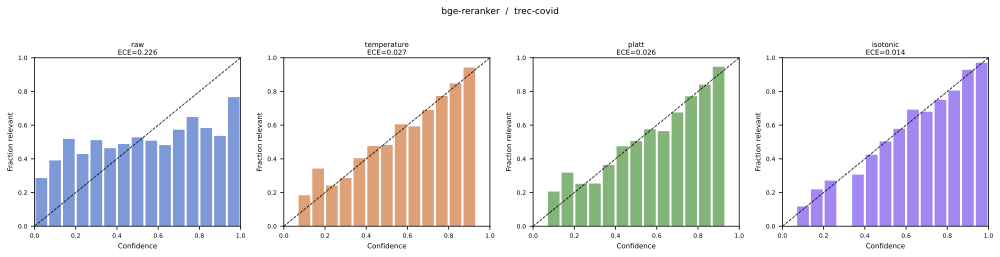
\includegraphics[width=\columnwidth]{paper_fig_bge_treccovid_4panel.png}
\caption{BGE on trec-covid (prevalence 0.62): raw, temperature, Platt, and
isotonic calibration. The progression from severe overconfidence to
near-diagonal bars is visible. This is a clean dataset, so the improvements
are genuine.}
\label{fig:fixworks}
\end{figure}

Crucially, none of the three methods disturb ranking quality. All are
monotone transforms, so they cannot reorder documents. The maximum absolute
change in nDCG@10 across all 45 pairs is $1.0 \times 10^{-4}$. Calibration
is, in a real sense, free.

% =============================================================================
\section{Discussion}
\label{sec:discussion}

\paragraph{Practical advice.}
If you consume sigmoid scores from these re-rankers as probabilities, the
short recommendation is: do not trust them raw. Temperature scaling is the
simplest fix, a one-line code change. The mean optimal temperature on clean
data ranges from about 8.5 (BGE) to 11.1 (TinyBERT). Where a held-out
calibration set with real negatives is available, Platt scaling is
substantially better (ECE roughly five times lower than temperature) and
isotonic regression is better still.

\paragraph{Platt scaling deserves more attention.}
One result that surprised us was how well Platt scaling performs. The single
extra parameter, an intercept that shifts the operating point, buys a
fivefold ECE improvement over temperature alone. On small calibration sets
where isotonic risks overfitting, Platt may be the pragmatic choice.

\paragraph{The methodological lesson.}
Report qrel prevalence whenever you measure calibration on BEIR. Restrict
method comparisons to datasets with genuine negatives. Our own naive
analysis demonstrates how convincingly wrong a pooled analysis can look:
temperature appears unreliable, isotonic appears magical, and neither
conclusion survives scrutiny.

% =============================================================================
\section{Limitations}
\label{sec:limits}

The clean subset is small: four datasets, one nearly single-class (scidocs,
prevalence 0.95), one with only 49 queries (webis-touche2020). Fifteen of 45
temperature values are lower bounds ($T {\geq} 20$). We studied only small
models (4M--278M); larger re-rankers and LLM-based re-rankers like
RankLLaMA~\cite{ma2024rankllama} may behave differently. All models were
trained on MS~MARCO. ECE itself depends on binning choices~\cite{nixon2019};
we fixed fifteen equal-width bins throughout.

% =============================================================================
\section{Conclusion}
\label{sec:conclusion}

Cross-encoder re-rankers are overconfident. Every model we tested, on every
domain where the measurement is valid, produces scores that are
systematically too high. The standard way to evaluate calibration on BEIR is
broken by positive-only judgments, creating misleading narratives about which
post-hoc fix to trust. When the evaluation is valid, all three methods work
and they are free: calibration improves without touching the ranking.
Isotonic regression leads, Platt is close behind and may suit small
calibration sets better, and temperature is the simplest option that still
helps substantially. We release scored data, fitted calibrators, and code at
\url{https://github.com/Codewithsayanjib/CalRank}.

% =============================================================================
\bibliographystyle{IEEEtran}
\begin{thebibliography}{20}

\bibitem{lewis2020rag} P.~Lewis et~al.,
``Retrieval-augmented generation for knowledge-intensive NLP tasks,''
\emph{NeurIPS}, 2020.

\bibitem{gao2024rag} Y.~Gao et~al.,
``Retrieval-augmented generation for large language models: A survey,''
\emph{arXiv:2312.10997}, 2024.

\bibitem{nguyen2016msmarco} T.~Nguyen et~al.,
``MS MARCO: A human generated machine reading comprehension dataset,''
\emph{NeurIPS Workshop}, 2016.

\bibitem{degroot1983} M.~H. DeGroot and S.~E. Fienberg,
``The comparison and evaluation of forecasters,''
\emph{The Statistician}, vol.~32, no.~1--2, pp.~12--22, 1983.

\bibitem{guo2017} C.~Guo, G.~Pleiss, Y.~Sun, and K.~Q. Weinberger,
``On calibration of modern neural networks,''
\emph{ICML}, 2017.

\bibitem{kadavath2022} S.~Kadavath et~al.,
``Language models (mostly) know what they know,''
\emph{arXiv:2207.05221}, 2022.

\bibitem{nogueira2019} R.~Nogueira and K.~Cho,
``Passage re-ranking with BERT,''
\emph{arXiv:1901.04085}, 2019.

\bibitem{wang2020minilm} W.~Wang et~al.,
``MiniLM: Deep self-attention distillation for task-agnostic compression of
pre-trained transformers,''
\emph{NeurIPS}, 2020.

\bibitem{jiao2020tinybert} X.~Jiao et~al.,
``TinyBERT: Distilling BERT for natural language understanding,''
\emph{Findings of EMNLP}, 2020.

\bibitem{clark2020electra} K.~Clark, M.-T. Luong, Q.~V. Le, and
C.~D. Manning,
``ELECTRA: Pre-training text encoders as discriminators rather than
generators,''
\emph{ICLR}, 2020.

\bibitem{xiao2023bge} S.~Xiao, Z.~Liu, P.~Zhang, and N.~Muennighoff,
``C-Pack: Packed resources for general Chinese embeddings,''
\emph{arXiv:2309.07597}, 2023.

\bibitem{thakur2021beir} N.~Thakur et~al.,
``BEIR: A heterogeneous benchmark for zero-shot evaluation of information
retrieval models,''
\emph{NeurIPS Datasets and Benchmarks}, 2021.

\bibitem{robertson2009bm25} S.~Robertson and H.~Zaragoza,
``The probabilistic relevance framework: BM25 and beyond,''
\emph{Found. Trends Inf. Retr.}, vol.~3, no.~4, pp.~333--389, 2009.

\bibitem{naeini2015} M.~P. Naeini, G.~F. Cooper, and M.~Hauskrecht,
``Obtaining well calibrated probabilities using Bayesian binning into
quantiles,''
\emph{AAAI}, 2015.

\bibitem{niculescu2005} A.~Niculescu-Mizil and R.~Caruana,
``Predicting good probabilities with supervised learning,''
\emph{ICML}, 2005.

\bibitem{platt1999} J.~Platt,
``Probabilistic outputs for support vector machines and comparisons to
regularized likelihood methods,''
\emph{Advances in Large Margin Classifiers}, 1999.

\bibitem{zadrozny2002} B.~Zadrozny and C.~Elkan,
``Transforming classifier scores into accurate multiclass probability
estimates,''
\emph{KDD}, 2002.

\bibitem{tian2023} K.~Tian et~al.,
``Just ask for calibration: Strategies for eliciting calibrated confidence
scores from language models fine-tuned with human feedback,''
\emph{EMNLP}, 2023.

\bibitem{desai2020} S.~Desai and G.~Durrett,
``Calibration of pre-trained transformers,''
\emph{EMNLP}, 2020.

\bibitem{craswell2020} N.~Craswell et~al.,
``Overview of the TREC 2020 Deep Learning Track,''
\emph{Proc. TREC}, 2020.

\bibitem{lin2021pyserini} J.~Lin et~al.,
``Pyserini: A Python toolkit for reproducible information retrieval research
with sparse and dense representations,''
\emph{SIGIR}, 2021.

\bibitem{ma2024rankllama} X.~Ma, L.~Gao, and J.~Callan,
``Fine-tuning LLaMA for multi-stage text retrieval,''
\emph{SIGIR}, 2024.

\bibitem{nixon2019} J.~Nixon et~al.,
``Measuring calibration in deep learning,''
\emph{CVPR Workshops}, 2019.

\end{thebibliography}

\end{document}
